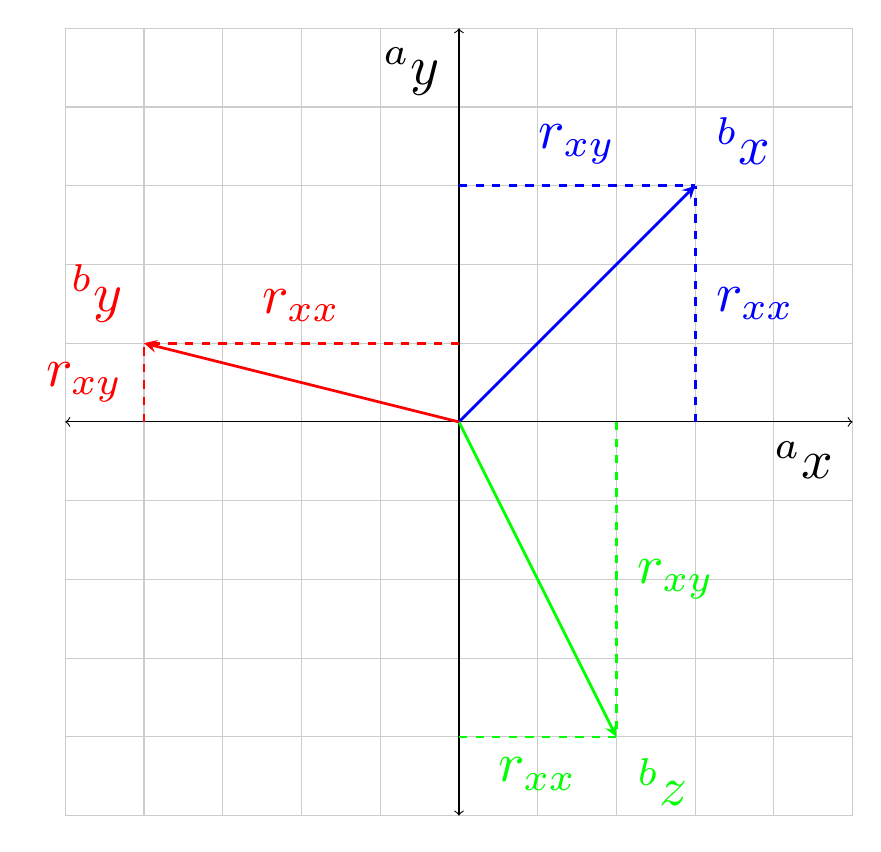
\begin{tikzpicture}
    \draw[thin,gray!40] (-5,-5) grid (5,5);
    \draw[<->] (-5,0)--(5,0) node[anchor=north east, scale=2]{$^{a}x$};
    \draw[<->] (0,-5)--(0,5) node[anchor=north east, scale=2]{$^{a}y$};
    \draw[line width=1pt,blue,-stealth](0,0)--(3,3) node[anchor=south west, scale=2]{$^{b}x$};
    \draw[line width=1pt,blue,dashed](3,0)--(3,3) node[midway, right, scale=2]{$r_{xx}$};
    \draw[line width=1pt,blue,dashed](0,3)--(3,3) node[midway, above, scale=2]{$r_{xy}$};
    \draw[line width=1pt,green,-stealth](0,0)--(2,-4) node[anchor=north west, scale=2]{${^{b}z}$};
    \draw[line width=1pt,green,dashed](0,-4)--(2,-4) node[midway, below, scale=2]{$r_{xx}$};
    \draw[line width=1pt,green,dashed](2,0)--(2,-4) node[midway, right, scale=2]{$r_{xy}$};
    \draw[line width=1pt,red,-stealth](0,0)--(-4,1) node[anchor=south east, scale=2]{${^{b}y}$};
    \draw[line width=1pt,red,dashed](0,1)--(-4,1) node[midway, above, scale=2]{$r_{xx}$};
    \draw[line width=1pt,red,dashed](-4,0)--(-4,1) node[midway, left, scale=2]{$r_{xy}$};
\end{tikzpicture}